%% body.tex -- Sections 1-5. All numbers trace to 01-VERIFIED-STATE.md or to
%% analysis/a1..a3 JSON files; experiment-dependent material is switched by
%% exp_results.tex.

\section{Introduction}
\label{sec:intro}

Sentiment classifiers for user reviews are usually trained on labels
that cost nothing: the star rating attached to each review. IMDb-style
corpora map high and low ratings to positive and negative and discard
the middle of the scale \citep{maas2011}, and the Amazon polarity
benchmark is built the same way \citep{zhang2015char}. The shortcut assumes
that a rating and the text beside it express the same thing. For
short reviews this is doubtful: a rating is an overall verdict, while
the text may praise one aspect, mock another, or say nothing
evaluative at all \citep{pang2005seeing}. Douban short reviews are an
extreme case (median 24 characters, frequently ironic), and the
assumption matters most for the three-way task, where the middle of
the scale cannot simply be dropped.

Two other cheap sources now compete with ratings. A small
human-labelled seed can train a model whose confident predictions
become pseudo-labels for the rest of the corpus
\citep{lee2013pseudo,xie2020selftraining}, and an LLM can annotate
text directly \citep{gilardi2023,tan2024survey}. Each is easy to
scale and each has a known weakness: pseudo-labels repeat the seed
model's errors, and LLM labels encode one model's conventions
\citep{moller2024parrot}. Which of them actually improves a
classifier, as judged by people rather than by more cheap labels, is
an empirical question, and it is the one this paper asks.

We work with a 910{,}998-review Douban corpus that has ratings but no
sentiment labels \citep{moviedata10m}, 600 gold labels from one film
page, and \emph{Human-400}, a 400-review test set labelled blind and
sharing no identifier with any training pool. Three questions
organise the study. \textbf{RQ1}: how well do star ratings represent
the sentiment expressed in review text, and does this depend on the
review population? \textbf{RQ2}: which supervision source improves a
classifier on blind human labels? \textbf{RQ3}: how much do label
provenance and model selection change the performance one reports?

Our findings are as follows.
\begin{itemize}[leftmargin=*,itemsep=1pt,topsep=2pt]
  \item \textbf{Ratings are a weak and population-dependent proxy.}
        A rating-derived label agrees with the semantic label on
        71.3\% of the single-film gold set but on only 51--62\% of
        corpus reviews. The corpus figure holds under four
        rating-blind annotators (one human, three LLMs), and
        agreement falls from 62--74\% for reviews over 100
        characters to 51--55\% for those of at most 20
        (\S\ref{sec:res-rating}).
  \item \textbf{LLM labels help where gold labels and pseudo-labels
        do not.} On Human-400, an ensemble built from the gold seed
        and its own pseudo-labels scores 55.8\%, the same as looking
        up the star rating. A MacBERT classifier fine-tuned on 17K
        LLM-labelled reviews reaches 64.3\%, and 64.8\% when fused
        with the ensemble ($+9.0$ points, McNemar $p{=}0.001$). With
        500 added labels, uniformly random and uncertainty-selected
        reviews give indistinguishable results
        (\S\ref{sec:res-human400}).
  \item \textbf{Label provenance changes the reported numbers.}
        Text classifiers score 23--28 points higher on LLM-consensus
        benchmark rows than on human-adjudicated ones, and
        cross-validated accuracy on the gold set drops from 89.5\%
        to 82.6--84.0\% once distillation targets and duplicate
        texts stop leaking across folds (\S\ref{sec:res-provenance}).
\end{itemize}
We release labels, identifiers, text hashes, prediction files and
analysis scripts for every table, with a datasheet-style description
of each artifact \citep{gebru2021,bender2018}.

\section{Related Work}
\label{sec:related}

\paragraph{Ratings as sentiment labels.}
\citet{pang2005seeing} treated rating prediction as a task distinct
from polarity classification, and standard benchmarks sidestep the
ambiguous middle of the scale by excluding it
\citep{maas2011,zhang2015char}. Surveys of the field
\citep{pang2008opinion,zhang2018dl} and recent LLM-era evaluations
\citep{zhang2024reality} largely take text-level labels as given. We
measure the rating--text gap directly on Chinese short reviews and
show that it varies with review length and population.

\paragraph{Weak and pseudo-supervision.}
Programmatic labelling \citep{ratner2017snorkel} and self-training
\citep{lee2013pseudo,xie2020selftraining} scale a small seed to a
large corpus, and a parallel literature models the resulting label
noise \citep{arazo2021pseudo,northcutt2021}. This work typically
evaluates on a fixed, trusted test split; we instead ask whether the
weak labels and the test labels can be trusted in the first place.

\paragraph{LLMs as annotators.}
Zero-shot LLMs can exceed crowd workers on some annotation tasks
\citep{gilardi2023}, their use as annotators is now widely studied
\citep{ding2023,tan2024survey}, and small models trained on LLM
labels inside an active-learning loop can be cost-effective
\citep{zhang2023llmaaa}. Two cautions recur. Classifiers trained on
LLM-generated data can trail those trained on human labels
\citep{moller2024parrot}, and showing annotators LLM suggestions
shifts the labels they produce and inflates measured LLM performance
\citep{schroeder2025humanloop}. Whether uncertainty-based selection
beats random sampling is itself unsettled \citep{settles2009,lowell2019}.
Our contribution is a comparison scored on blind human labels, with a
budget-matched random-selection control.

\paragraph{Evaluation validity.}
Train--test overlap inflates NLP results \citep{elangovan2021}, as do
benchmark contamination \citep{sainz2023contamination,balloccu2024},
leakage through preprocessing and model selection
\citep{kapoor2023,cawley2010}, and under-reported annotation
procedures \citep{kunilovskaya2026,alkhalifa2026}. On subjective
tasks, disagreement between annotators carries signal
\citep{davani2022,plank2022}. We follow \citet{dror2018hitchhiker}
for significance testing and report every result by label provenance.

\section{Data}
\label{sec:data}

The task is three-way sentiment classification (positive, neutral,
negative) of Douban movie short reviews. Table~\ref{tab:datasets}
lists the datasets; Appendix~\ref{app:annotation} gives the annotation
guidelines, which define \emph{neutral} as the absence of a
discernible overall lean (mixed at parity, purely descriptive, or
off-topic text).

\begin{table}[t]
\centering
\small
\setlength{\tabcolsep}{3pt}
\begin{tabular}{@{}lrp{2.55cm}l@{}}
\toprule
Dataset & Rows & Semantic labels & Role \\
\midrule
Gold-600 & 600 & human & seed; CV \\
Corpus & 910{,}998 & none (ratings only) & unlabelled \\
LLM-17K & 16{,}906 & 15{,}906 LLM; 721 LLM consensus; 279 human-adjudicated & training \\
Dev-1000 & 1{,}000 & 800 LLM consensus; 200 human-adjudicated & selection \\
Human-400 & 400 & blind human & test \\
\bottomrule
\end{tabular}
\caption{Datasets. Every row except Gold-600 is drawn from the corpus.
Dev-1000 is a development set, not a test set.}
\label{tab:datasets}
\end{table}

\paragraph{Gold-600.} We collected the first 30 comment pages of one
Douban film: 600 rows, 592 unique texts, mean length 111 characters.
The authors assigned each a semantic label under written guidelines
(316 positive, 92 neutral, 192 negative). A second, rating-derived
label follows the usual rule (4--5 stars positive, 3 neutral, 1--2
negative); 14 rows have no rating.

\paragraph{Corpus.} Cleaning and deduplicating the 4.43M comments of
Moviedata-10M \citep{moviedata10m} leaves 910{,}998 reviews of
20{,}966 films by 249{,}105 users, with ratings but no sentiment
labels.

\paragraph{LLM-17K.} We selected 16{,}906 corpus reviews on which a
MacBERT student trained on Gold-600 was uncertain (top-two margin
band, entropy, and disagreement between students) and labelled
15{,}906 of them zero-shot with DeepSeek-V4.1-Flash. The remaining 1{,}000 carry labels from the same two-pass
procedure described next, including author adjudication under the
same interface that showed ratings and a model prediction. All
LLM-17K rows are text-disjoint from every evaluation set.

\paragraph{Dev-1000.} One thousand corpus reviews sampled uniformly
at random were labelled twice by one LLM annotator with different
few-shot examples, blind to ratings; the passes agree on 86.7\%
($\kappa{=}0.80$). Disagreements and a sample of agreements (200 rows)
were adjudicated by an author with the star rating and a model
prediction visible; the other 800 rows keep the consensus label. We used Dev-1000 for every
design decision, so its numbers are development estimates. A further
500 uniformly sampled reviews with DeepSeek labels (\emph{Fresh-500})
serve as a replication sample in \S\ref{sec:res-rating} and as the
random arm in \S\ref{sec:res-human400}.

\paragraph{Human-400.} For a test set that no system had seen, we
sampled 400 corpus reviews after removing every identifier used
anywhere else in the project, including the pool of reviews that the
Gold-600 student labels with confidence $\geq 0.7$ (about 30\% of the
corpus). The sample is stratified by length (160, 120, 80 and 40
reviews of $\leq$20, 21--50, 51--100 and $>$100 characters). One
author labelled it without seeing ratings or model output: 156
positive, 179 neutral, 65 negative. The 400 reviews span 390 distinct
films and 393 users, so film- or user-level clustering does not
inflate the intervals. A text-level audit against
462{,}879 training-pool texts found no exact or near-duplicate match
(Appendix~\ref{app:human400}).
\ifSfive A second annotator independently re-labelled all 400 reviews
under the same guidelines; raw agreement is \IAAraw\% (Cohen's
$\kappa{=}\IAAkappa$, 95\% CI \IAAkappaCI). We score systems against
the first annotator and report the second as a robustness check.\fi
Two properties bound what Human-400 can show: it is not a uniform
sample, and it covers the part of the corpus where gold-only
supervision is least confident. We return to both in
\S\ref{sec:res-human400}.

\section{Systems and Protocol}
\label{sec:method}

\paragraph{Rating lookup.} The rule above applied to the review's own
star rating. It uses information the text classifiers do not have and
needs no training.

\paragraph{GoldEns (gold-only ensemble).} Our strongest system built
without LLM labels combines a MacBERT-base classifier
\citep{cui2020macbert} trained on Gold-600 with a small MLP on frozen
features of a 1.3B-parameter Chinese sentiment encoder
\citep{fengshenbang2022}, blended 1:2, plus a neutral-probability
correction that draws on a detector trained on 115K corpus
pseudo-labels produced by the Gold-600 student. It is the result of
about twenty rejected variants (Appendix~\ref{app:negative}) and uses
both gold labels and pseudo-labels. Appendix~\ref{app:goldens} gives
its equations.

\paragraph{LLM-label student.} A single MacBERT-base classifier
fine-tuned with cross-entropy on Gold-600 plus LLM-17K (4 epochs,
learning rate $2{\times}10^{-5}$, batch 32, maximum length 256). We
average the probabilities of five seeds. \emph{Mix} is
$0.6\,P_{\text{student}} + 0.4\,P_{\text{GoldEns}}$, with the weight
chosen on Dev-1000 and then frozen.

\paragraph{Zero-shot LLMs.} Qwen3-4B \citep{qwen2025} scores the three
labels by log-probability, run locally.
\ifSone DeepSeek-V4.1-Flash, the teacher that labelled LLM-17K, is
run with the labelling prompt.\fi

\ifStwo
\paragraph{Label-source swap.} To separate the label source from the
choice of texts, we retrain the student on the \emph{same} 16{,}906
reviews with their labels replaced by (i) the rating rule or (ii) the
Gold-600 student's own predictions, holding the recipe and seeds
fixed.
\fi

\paragraph{Evaluation.} We report accuracy, macro-F1 and neutral
recall for the three-way task, and accuracy on the non-neutral rows
for the binary task (dedicated binary models where available).
Intervals are 95\% Wilson intervals; paired comparisons use exact
McNemar tests with Holm correction over the pairwise Human-400
comparisons tabulated in Appendix~\ref{app:human400}. Intervals are
conditional on the released seed ensembles; per-seed spreads are in
Appendix~\ref{app:human400}. No configuration was tuned on Human-400.

\section{Results}
\label{sec:results}

\subsection{RQ1: What do star ratings encode?}
\label{sec:res-rating}

\begin{table}[t]
\centering
\small
\setlength{\tabcolsep}{2.5pt}
\begin{tabular}{@{}llrcr@{}}
\toprule
Sample & Labels from & $n$ & Agree (\%) & 3$\star$ neu. \\
\midrule
Gold-600 & human & 586 & 71.3 {\scriptsize[67.5, 74.8]} & 30.6 \\
\midrule
Human-400 & blind human & 400 & 55.8 {\scriptsize[50.9, 60.5]} & 56.8 \\
Dev-1000 & released & 1000 & 62.2 {\scriptsize[59.2, 65.2]} & 43.6 \\
\quad adjudicated & human & 200 & 61.0 {\scriptsize[54.1, 67.5]} & 56.3 \\
Dev-1000 & LLM, one pass & 1000 & 58.3 {\scriptsize[55.2, 61.3]} & 46.0 \\
Dev-1000 & DeepSeek-Flash & 992 & 57.3 {\scriptsize[54.2, 60.3]} & 55.0 \\
Dev-1000 & Qwen3-4B & 1000 & 51.5 {\scriptsize[48.4, 54.6]} & 47.2 \\
Fresh-500 & DeepSeek-Flash & 500 & 53.4 {\scriptsize[49.0, 57.7]} & 51.3 \\
\bottomrule
\end{tabular}
\caption{Agreement between the rating rule and semantic labels, with
95\% Wilson intervals, and the share of three-star reviews labelled
neutral. All annotators below the first rule labelled corpus reviews
without seeing ratings, except the adjudicated row: that human
adjudicator saw the rating and a model prediction. DeepSeek-Flash
returned a parseable label for 992 of the 1{,}000 Dev-1000 rows.}
\label{tab:stars}
\end{table}

\begin{figure}[t]
\centering
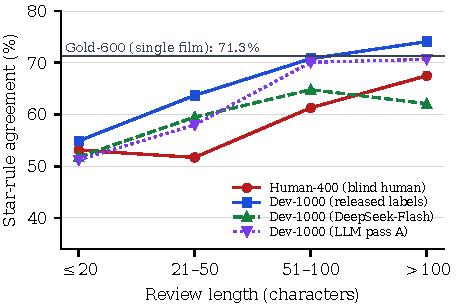
\includegraphics[width=0.92\columnwidth]{fig_star_length.pdf}
\caption{Rating-rule agreement by review length. The solid grey line
is Gold-600, whose reviews average 111 characters.}
\label{fig:star-length}
\end{figure}

On Gold-600 the rating rule agrees with the human semantic label on
71.3\% of rated rows (Table~\ref{tab:stars}). Agreement is high at
the extremes (94.3\% at one star, 96.9\% at five) and collapses in
the middle: only 30.6\% of three-star reviews are semantically
neutral, and 51.3\% are negative.

\begin{table}[t]
\centering
\small
\setlength{\tabcolsep}{3.5pt}
\begin{tabular}{@{}crrrrrrrr@{}}
\toprule
 & \multicolumn{4}{c}{Gold-600} & \multicolumn{4}{c}{Human-400} \\
\cmidrule(lr){2-5}\cmidrule(l){6-9}
$\star$ & $n$ & pos & neu & neg & $n$ & pos & neu & neg \\
\midrule
5 & 130 & \textbf{96.9} & 3.1 & 0.0 & 67 & \textbf{62.7} & 32.8 & 4.5 \\
4 & 197 & \textbf{78.7} & 12.7 & 8.6 & 138 & \textbf{50.7} & 44.9 & 4.3 \\
3 & 160 & 18.1 & \textbf{30.6} & 51.3 & 132 & 28.0 & \textbf{56.8} & 15.2 \\
2 & 64 & 0.0 & 14.1 & \textbf{85.9} & 39 & 17.9 & 38.5 & \textbf{43.6} \\
1 & 35 & 0.0 & 5.7 & \textbf{94.3} & 24 & 0.0 & 20.8 & \textbf{79.2} \\
\bottomrule
\end{tabular}
\caption{Human semantic labels by star rating (\%). Bold marks the
class the rating rule assigns.}
\label{tab:perstar}
\end{table}

The corpus looks different (Table~\ref{tab:perstar}). On Human-400 agreement is 55.8\%, and the
three-star pattern reverses: 56.8\% of three-star reviews are neutral
and 15.2\% negative ($\chi^2{=}41.8$, $p{<}10^{-9}$ against the
Gold-600 distribution). Four-star agreement falls from 78.7\% to
50.7\%. Because Human-400 has one annotator, we repeat the
measurement with every other rating-blind label source we have. On
uniform corpus samples, agreement is 62.2\% with the released
Dev-1000 labels (itself 80\% LLM consensus) and 51.5--58.3\% with
three different LLM annotators; no source reaches
the Gold-600 figure, and all put the neutral share of three-star
reviews between 44\% and 57\%. At corpus scale, the Gold-600
student's predictions agree with the rating rule on 47.8\% of all
910{,}998 reviews.

Length explains much of the difference
(Figure~\ref{fig:star-length}). Under the four label sources shown,
agreement is 51--55\% for reviews of at most 20 characters and
62--74\% above 100 characters. Gold-600 reviews are long, and a long
review usually states its verdict; a ten-character review often does
not, and is labelled neutral whatever its rating (55.0\% of Human-400
reviews of at most 20 characters are neutral, against 25.0\% of those
above 100). Length is not the whole story: among Human-400 reviews
longer than 50 characters, 47.5\% of three-star reviews are neutral
and 20.0\% negative, still unlike Gold-600, so the mid-scale
reviewers of that one film appear unusually negative.

Ratings therefore mislabel between 38\% and 49\% of corpus reviews
for the three-way task, depending on who supplies the semantic label. They remain informative: a rating lookup is a
baseline that any text classifier in this setting should be required
to beat, and the next section shows that this is not automatic.

\subsection{RQ2: Which supervision helps on Human-400?}
\label{sec:res-human400}

\begin{table}[t]
\centering
\small
\setlength{\tabcolsep}{2.6pt}
\begin{tabular}{@{}lcccc@{}}
\toprule
 & \multicolumn{3}{c}{Three-way ($n{=}400$)} & Bin. \\
\cmidrule(lr){2-4}
System & Acc.\ {\scriptsize[95\% CI]} & F1 & Neu.R & Acc. \\
\midrule
Rating lookup & 55.8 {\scriptsize[50.9, 60.5]} & 55.5 & 41.9 & 83.7 \\
\midrule
\multicolumn{5}{@{}l}{\emph{Gold labels and pseudo-labels only}} \\
Gold-600 student & 52.8 {\scriptsize[47.9, 57.6]} & 49.3 & -- & 69.2$^\ast$ \\
GoldEns & 55.8 {\scriptsize[50.9, 60.5]} & 55.4 & 50.3 & 76.5 \\
\midrule
\multicolumn{5}{@{}l}{\emph{Gold-600 plus LLM labels}} \\
$+$500 random & 60.5 {\scriptsize[55.6, 65.2]} & 56.9 & -- & 79.2 \\
$+$500 uncertain & 61.3 {\scriptsize[56.4, 65.9]} & 55.3 & -- & 77.4 \\
$+$LLM-17K (student) & 64.3 {\scriptsize[59.4, 68.8]} & 62.1 & \textbf{76.0} & 83.7 \\
Mix & \textbf{64.8} {\scriptsize[59.9, 69.3]} & \textbf{63.5} & 73.7 & 83.7 \\
\ifStwo
\midrule
\multicolumn{5}{@{}l}{\emph{Same 16.9K texts, other labels}} \\
$+$rating-rule labels & \SwapStarAcc\ {\scriptsize\SwapStarCI} & \SwapStarF & \SwapStarNeuR & \SwapStarBin \\
$+$student pseudo-labels & \SwapPseudoAcc\ {\scriptsize\SwapPseudoCI} & \SwapPseudoF & \SwapPseudoNeuR & \SwapPseudoBin \\
\fi
\midrule
\multicolumn{5}{@{}l}{\emph{Zero-shot LLMs}} \\
Qwen3-4B & 61.5 {\scriptsize[56.6, 66.1]} & 59.0 & 70.4 & -- \\
\ifSone
DeepSeek-V4.1-Flash & \DSFlashAcc\ {\scriptsize\DSFlashCI} & \DSFlashF & \DSFlashNeuR & \DSFlashBin \\
\fi
\midrule
\multicolumn{5}{@{}l}{\emph{Feature baseline}} \\
TF-IDF$+$LR & 60.5 {\scriptsize[55.6, 65.2]} & 58.7 & 79.3 & 45.3 \\
\bottomrule
\end{tabular}
\caption{Human-400 results (\%). F1 is macro-F1; Neu.R is neutral
recall; Bin.\ is accuracy on the 221 non-neutral reviews
($^\ast$three-way model with the neutral class marginalised out). The
binary rating rule maps 1--2 stars to negative and the rest to
positive.}
\label{tab:human400}
\end{table}

\paragraph{Gold labels and pseudo-labels do not beat the rating.}
GoldEns reaches 89.5\% in naive cross-validation on Gold-600 and
82.6--84.0\% after the corrections of \S\ref{sec:res-provenance}. On
Human-400 it scores 55.8\% (Table~\ref{tab:human400}): 223 of 400
correct, the same count as the rating lookup, although the two err on
different reviews (94 discordant pairs each way). Its MacBERT
component alone scores 52.8\%. On the binary task GoldEns is below
the rating rule (76.5\% against 83.7\%). The ensemble's errors
concentrate in the neutral class, where it recovers half of the
neutral reviews and predicts negative for 66 of them; the neutral
convention learned from 92 single-film examples does not carry over
to short corpus reviews.

\paragraph{LLM labels help.}
Fine-tuning the same MacBERT architecture on Gold-600 plus LLM-17K
gives 64.3\%, and Mix gives 64.8\%, 9.0 points above both GoldEns and
the rating lookup. The gain over GoldEns is significant (exact
McNemar $p{=}0.0013$; Holm-adjusted $p{=}0.021$ over the 16 pairwise
Human-400 tests). The gain over the rating lookup is nominally
significant ($p{=}0.0074$) but does not survive correction (adjusted
$p{=}0.10$), and fusion adds nothing reliable to the student alone
($p{=}0.85$): the 1.3B-parameter ensemble is not needed for the
result. The improvement is a repair of the neutral class. Neutral
recall rises from 50.3\% to 73.7\% and negative precision from
35.3\% to 54.4\%, at the cost of negative recall (81.5\% to 66.2\%).
It is not uniform: on the 30 reviews the annotator flagged as mixed,
Mix scores 40.0\% against 53.3\% for GoldEns. On the binary task the
student matches the rating rule (83.7\% each, with a more balanced
error profile: macro-F1 81.3 against 77.9) and improves on GoldEns
by 7.2 points ($p{=}0.026$, adjusted $0.29$).

\ifStwo
\paragraph{Same texts, different labels.}
Relabelling the same 16{,}906 reviews with the rating rule gives
\SwapStarAcc\% and with the Gold-600 student's own predictions
\SwapPseudoAcc\% (McNemar against the LLM-labelled student:
$p{=}\SwapStarVsLLMP$ and $p{=}\SwapPseudoVsLLMP$). \StwoInterp
\fi

\paragraph{Zero-shot LLMs.}
Qwen3-4B, with no task training, reaches 61.5\%, above GoldEns and
below Mix; neither difference is significant after correction (raw
$p{=}0.079$ and $0.26$).
\ifSone DeepSeek-V4.1-Flash, the model that produced most of the
training labels, scores \DSFlashAcc\% (against Mix: McNemar
$p{=}\DSFlashVsMixP$). \SoneInterp
\else We did not run the commercial teacher on Human-400, so we
cannot say how much of the teacher's accuracy the student
retains.\fi

\paragraph{Feature baseline.}
A TF-IDF character n-gram logistic regression trained on the same
Gold-600\,+\,LLM-17K labels reaches 60.5\% (macro-F1 58.7), below
every neural system but not significantly different from Mix after
correction ($p{=}0.18$): part of Human-400's difficulty is intrinsic
to the items rather than the model class.

\paragraph{Scale, not selection.}
LLM-17K was chosen by uncertainty, which raises the question of
whether the gain comes from the selection rule or from the volume.
We can test this at one budget. Adding 500 uniformly sampled
DeepSeek-labelled reviews (Fresh-500) to Gold-600 gives 60.5\%;
adding the first 500 uncertainty-selected reviews gives 61.3\%
(McNemar $p{=}0.83$; bootstrap 95\% CI for the difference
$[-3.8, +5.3]$ points), in line with reports that active learning
does not reliably beat random sampling
\citep{lowell2019}. Five hundred LLM labels of either kind recover
more than half of the gain that 17K give over either gold-only
system.
\ifSthree \CurveSentence
\else On Dev-1000 accuracy rises with pool size, from 72.0\% at 1K to
77.1\% at 17K against 65.0\% for GoldEns
(Figure~\ref{fig:al-scaling}), but each point there is a
selected configuration scored largely on LLM labels.\fi
\ Teacher quality matters at fixed size: with 11K labels, a
Qwen3-4B teacher gives 72.4\% on Dev-1000 against 74.9\% for
DeepSeek.

\begin{figure}[t]
\centering
\ifSthree
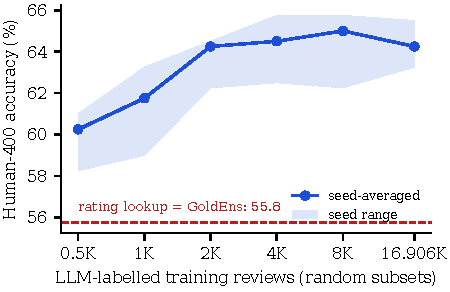
\includegraphics[width=0.9\columnwidth]{fig_h400_curve.pdf}
\caption{Human-400 accuracy of the LLM-label student against the
number of LLM-labelled training reviews (random subsets of LLM-17K;
mean and range over seeds). Dashed lines: rating lookup and GoldEns.}
\else
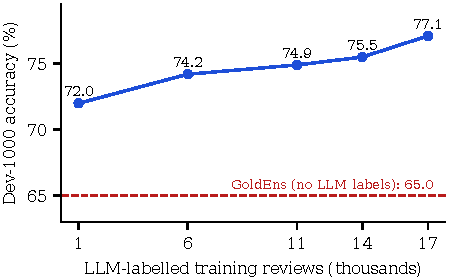
\includegraphics[width=0.85\columnwidth]{fig3_al_scaling.pdf}
\caption{Three-way accuracy on Dev-1000 (development set) against the
number of LLM-labelled training reviews, for the student fused with
GoldEns. Every point is a selected configuration.}
\fi
\label{fig:al-scaling}
\end{figure}

\paragraph{Scope.}
Human-400 excludes reviews on which the Gold-600 student is
confident, which disadvantages gold-only systems. On Dev-1000, a
uniform sample, that student agrees with the released label on
73.4\% of the 29\% of reviews in its confident band and on 45--63\%
of the rest, while the rating rule scores 61--63\% in every band.
GoldEns would therefore score higher on a uniform sample than on
Human-400, and we do not claim that it merely equals a rating lookup
corpus-wide. The claim Human-400 supports is narrower: on the
reviews where a gold-seeded model is unsure, which are about 70\% of
the corpus, LLM labels improve on it and gold-derived pseudo-labels
do not.

\subsection{RQ3: How much does provenance move the numbers?}
\label{sec:res-provenance}

\begin{table}[t]
\centering
\small
\setlength{\tabcolsep}{3.2pt}
\begin{tabular}{@{}lrcccc@{}}
\toprule
Dev-1000 rows & $n$ & Rating & GoldEns & Mix & DS-Flash \\
\midrule
All & 1000 & 62.2 & 65.0 & 77.1 & 82.0 \\
LLM consensus & 800 & 62.5 & 69.6 & 82.4 & 87.5 \\
Human-adjudicated & 200 & 61.0 & 46.5 & 56.0 & 59.5 \\
\bottomrule
\end{tabular}
\caption{Three-way accuracy (\%) on Dev-1000 by label provenance.
DS-Flash is DeepSeek-V4.1-Flash zero-shot, scored on its 992, 797 and
195 parseable rows. Mix was selected on this set.}
\label{tab:dev}
\end{table}

\paragraph{Who labelled the benchmark.}
Table~\ref{tab:dev} splits Dev-1000 by label provenance. Every text
model scores 23--28 points lower on the 200 human-adjudicated rows
than on the 800 LLM-consensus rows, and the systems closest to the
LLM labels gain most from them: on consensus rows Mix leads GoldEns
by 12.8 points and the rating lookup by 19.9; on adjudicated rows the
rating lookup, which is indifferent to how hard the text is, is level
with the LLM teacher (61.0\% against 59.5\%) and ahead of Mix. The adjudicated rows are not a fair sample. They are mostly
reviews on which two LLM passes disagreed, so the split confounds
label source with difficulty, and they were adjudicated with the star
rating and a model prediction on screen, the setting in which
\citet{schroeder2025humanloop} find that labels drift toward the
suggestion. The two LLM passes agree on 33.5\% of these rows against
100\% of consensus rows by construction. The practical point stands
either way: a benchmark whose labels are mostly LLM consensus rewards
agreement with LLM conventions, and its headline number (77.1\% for
Mix) is far from what blind human labels give (64.8\%).

\paragraph{What the folds leaked.}
GoldEns was first evaluated by five-fold cross-validation on Gold-600
at 89.5\% accuracy (95.9\% binary). Three channels inflate that
figure (Table~\ref{tab:oof}; Appendix~\ref{app:audit}). The
distillation targets used to train each fold's models came from
teachers that had seen the held-out fold; retraining with hard labels
only removes 5.5 points. The neutral detector was trained on
pseudo-labels from a student fitted to all 600 rows; dropping it
removes 0.7. Eight duplicated texts could fall on both sides of a
split; deduplicating removes about one more. None of these is a bug
in the cross-validation code, and none shows up without tracing
where each training signal came from. The corrected range,
82.6--84.0\%, is still far above the 55.8\% that the same system
scores on Human-400, which is a difference of population rather than
of leakage.

\begin{table}[t]
\centering
\small
\setlength{\tabcolsep}{4pt}
\begin{tabular}{@{}lcc@{}}
\toprule
GoldEns, Gold-600 cross-validation & 3-way & Binary \\
\midrule
As first evaluated & 89.5 & 95.9 \\
Hard labels only (no teacher targets) & 84.0 & 92.9 \\
\quad and no pseudo-label detector & 83.3 & -- \\
\quad and 592 unique texts & 82.6--83.1 & 91.5 \\
\bottomrule
\end{tabular}
\caption{Out-of-fold accuracy (\%) of GoldEns as leakage channels are
removed. The binary pipeline has no pseudo-label detector. The last
row gives the range with the detector kept or removed.}
\label{tab:oof}
\end{table}

\paragraph{Selection.}
All design choices for the LLM-label student (pool size, teacher,
epochs, seeds, fusion weight) were read off Dev-1000 across 26
mixture configurations and about 73 training runs, and 68.7\% of
Dev-1000 rows occur in earlier corpus-derived training pools (none in
LLM-17K). We estimate the resulting optimism at 0.3--1.0 points
(Appendix~\ref{app:audit}), small beside the provenance effect above,
and it does not touch Human-400, on which nothing was selected.
